\documentclass[tikz,border=10pt]{standalone}
\usepackage{amsmath,amssymb}
\usetikzlibrary{arrows.meta,positioning,calc}

\begin{document}
	
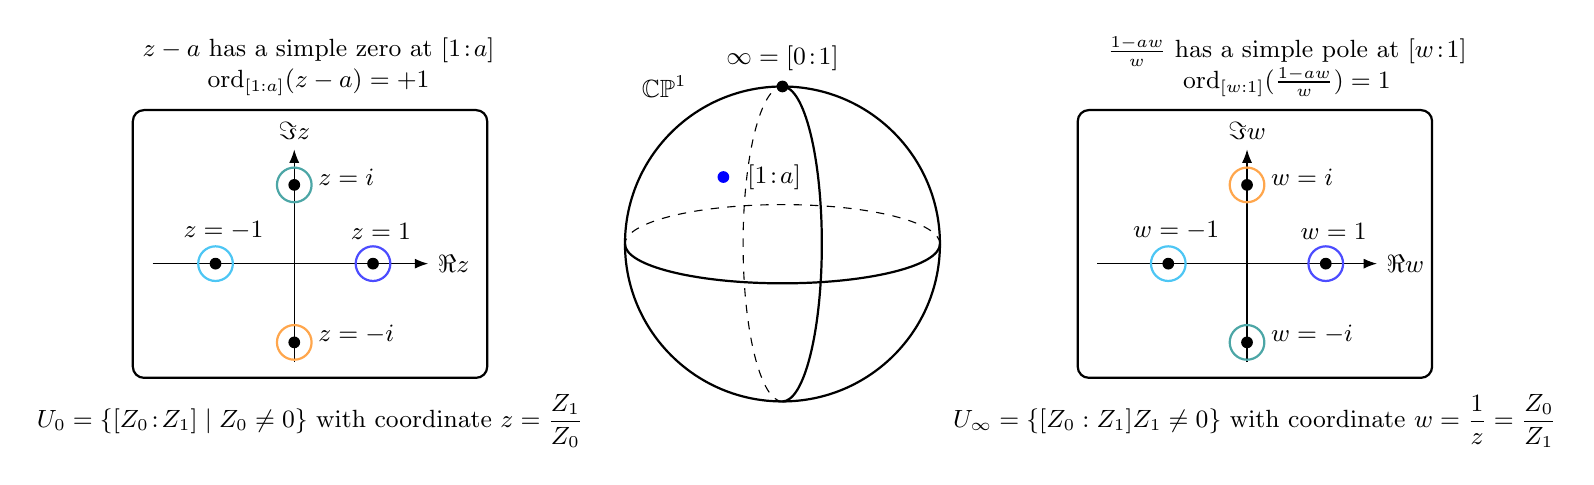
\begin{tikzpicture}[
	>=Latex,
	font=\small,
	point/.style={circle,fill=black,inner sep=1.5pt},
	box/.style={draw,rounded corners,thick,minimum width=4.5cm,minimum height=3.4cm},
	note/.style={align=left}
	]
	
	%------------------------------------------------
	% Left box: U_0 chart
	%------------------------------------------------
	\node[box] (L) at (-6,0) {};
	\node[anchor=north] at ([yshift=-35mm]L.north) {$U_0=\{[Z_0\!:\!Z_1]\mid Z_0\neq 0\}$ with coordinate $z=\dfrac{Z_1}{Z_0}$};
	
	% axes
	\draw[->] (-8,-.25) -- (-4.5,-.25) node[right] {$\Re z$};
	\draw[->] (-6.2,-1.5) -- (-6.2,1.2) node[above] {$\Im z$};
	
	\node[point,label={[xshift=1mm,yshift=1mm]above:$z=1$}] at (-5.2,-.25) {};
	\draw[thick,blue!70] (-5.2,-0.25) circle (0.22);
	\node[point,label={[xshift=1mm,yshift=1mm]above:$z=-1$}] at (-7.2,-.25) {};
	\draw[thick,cyan!70] (-7.2,-0.25) circle (0.22);
	
	\node[point,label={[xshift=1mm,yshift=1mm]right:$z=i$}] at (-6.2,.75) {};
	\draw[thick,teal!70] (-6.2,.75) circle (0.22);
	\node[point,label={[xshift=1mm,yshift=1mm]right:$z=-i$}] at (-6.2,-1.25) {};
	\draw[thick,orange!70] (-6.2,-1.25) circle (0.22);
	
%	% point a
%	\node[point,label={[xshift=1mm,yshift=1mm]right:$z=a$}] (a0) at (-6.1,-0.8) {};
%	\draw[thick,blue!70] (-6.1,-0.8) circle (0.22);
	\node[note,anchor=west,align=center] at (-8.25,2.25) {
		$z-a$ has a simple zero at $[1\!:\!a]$\\
		$\operatorname{ord}_{[1:a]}(z-a)=+1$};
				
	%------------------------------------------------
	% Middle: CP^1 picture
	%------------------------------------------------
	\node at (-1.5,2) {$\mathbb{CP}^1$};
	
	% sphere / projective line picture
	\draw[thick] (0,0) circle (2);
	\draw[thick] (-2,0) arc[start angle=180,end angle=360,x radius=2,y radius=0.5];
	\draw[dashed] (2,0) arc[start angle=0,end angle=180,x radius=2,y radius=0.5];
	\draw[thick] (0,2) arc[start angle=90,end angle=-90,x radius=.5,y radius=2];
	\draw[dashed] (0,-2) arc[start angle=270,end angle=90,x radius=.5,y radius=2];
	
	% top point = infinity
	\node[point,label={[yshift=0mm]above:$\infty=[0\!:\!1]$}] (inf) at (0,2) {};
	
	% finite point [1:a]
	\node[point,blue,label={[xshift=1mm]right:$[1\!:\!a]$}] (pa) at (-0.75,0.85) {};
		
%	% chart labels on sphere
%	\node at (0,-1.95) {$U_0$};
%	\node at (0,1.1) {$U_\infty=\{[Z_0\!:\!Z_1]\mid Z_1\neq 0\}$};
		
%	% zero/pole labels
%	\node[blue!70!black] at (1.65,-1.35) {zero of order $1$};
%	\node[red!75!black] at (1.4,1.45) {pole of order $1$};
		
%	% arrows from side charts
%	\draw[->,thick] (-3.7,0) .. controls (-2.5,0.2) and (-1.3,-0.4) .. (pa);
%	\draw[->,thick] (3.7,0) .. controls (2.5,0.4) and (1.2,1.1) .. (inf);
		
	%------------------------------------------------
	% Right box: U_infty chart
	%------------------------------------------------
	\node[box] (R) at (6,0) {};
	\node[anchor=north] at ([yshift=-35mm]R.north) {$U_\infty=\{[Z_0:Z_1]Z_1\neq 0\}$ with coordinate $w=\dfrac{1}{z}=\dfrac{Z_0}{Z_1}$};
		
	% local disk around w=0
	\draw[->] (4,-0.25) -- (7.55,-0.25) node[right] {$\Re w$};
	\draw[->] (5.9,-1.5) -- (5.9,1.2) node[above] {$\Im w$};
	
	\node[point,label={[xshift=1mm,yshift=1mm]above:$w=1$}] (w0) at (6.9,-0.25) {};
	\draw[thick,blue!70] (6.9,-0.25) circle (0.22);
	
	\node[point,label={[xshift=1mm,yshift=1mm]above:$w=-1$}] at (4.9,-.25) {};
	\draw[thick,cyan!70] (4.9,-0.25) circle (0.22);
	
	\node[point,label={[xshift=1mm,yshift=1mm]right:$w=i$}] at (5.9,.75) {};
	\draw[thick,orange!70] (5.9,.75) circle (0.22);
	\node[point,label={[xshift=1mm,yshift=1mm]right:$w=-i$}] at (5.9,-1.25) {};
	\draw[thick,teal!70] (5.9,-1.25) circle (0.22);
		
%	\node[note,anchor=west] at (5.45,0.7) {$z=\dfrac{1}{w}$};
%	\node[note,anchor=west] at (5.45,0.15) {$z-a=\dfrac{1-aw}{w}$};
%	\node[note,anchor=west] at (5.45,-0.45) {$1-aw$ is a unit at $w=0$};
%	\node[note,anchor=west] at (5.45,-1.2) {$\operatorname{ord}_{\infty}(z-a)=-1$};
		
	\node[note,anchor=west,align=center] at (4,2.25) {
		$\frac{1-aw}{w}$ has a simple pole at $[w\!:\!1]$\\
		$\operatorname{ord}_{[w:1]}(\frac{1-aw}{w})=1$};
		
	%------------------------------------------------
	% Bottom divisor statement
	%------------------------------------------------
%	\node[draw,rounded corners,fill=gray!8,inner sep=6pt,align=center] at (0,-3.15)
%	{
%			$\displaystyle \operatorname{div}(z-a)=[a]-[\infty]$
%			\\[2mm]
%			simple zero at $[1\!:\!a]$ \qquad and \qquad simple pole at $\infty$
%		};
		
\end{tikzpicture}
\end{document}